% =====================================================================
% RESPIRATECH: INTELLIGENT IoT AND AI-BASED BREATH ANALYZER
% FOR EARLY DISEASE PREDICTION IN HEALTHCARE
% VTU Mini Project Report - LaTeX Source
% Department of Computer Science and Engineering
% (IoT, CyberSecurity including Blockchain)
% Alva's Institute of Engineering & Technology, Moodbidri
% Academic Year: 2025-2026
% =====================================================================

\documentclass[12pt,a4paper]{report}
\usepackage[left=1.25in,right=1in,top=1in,bottom=1in]{geometry}
\usepackage{times}
\usepackage{graphicx}
\usepackage{fancyhdr}
\usepackage{titlesec}
\usepackage{setspace}
\usepackage{hyperref}
\usepackage{enumitem}
\usepackage{array}
\usepackage{longtable}
\usepackage{xcolor}
\usepackage{tikz}
\usepackage{background}
\usepackage{ulem}
\usepackage{tabularx}
\usepackage{multirow}
\usepackage{caption}

\onehalfspacing

% ===================== COLOR DEFINITIONS =====================
\definecolor{darkred}{RGB}{139,0,0}
\definecolor{darkblue}{RGB}{0,0,139}
\definecolor{darkgreen}{RGB}{0,128,0}

% ===================== PAGE BORDER (Front Matter Only) =====================
\newcommand{\enableborder}{%
\backgroundsetup{
  scale=1,
  color=black,
  opacity=1,
  angle=0,
  position=current page.center,
  vshift=0cm,
  hshift=0cm,
  contents={%
    
\begin{tikzpicture}[remember picture, overlay]
      \draw[black, line width=2pt] 
        ([shift={(0.5cm,-0.5cm)}]current page.north west) 
        rectangle 
        ([shift={(-0.5cm,0.5cm)}]current page.south east);
      \draw[black, line width=0.5pt] 
        ([shift={(0.65cm,-0.65cm)}]current page.north west) 
        rectangle 
        ([shift={(-0.65cm,0.65cm)}]current page.south east);
    \end{tikzpicture}%
  }
}}
\newcommand{\disableborder}{%
\backgroundsetup{contents={}}%
}

% ===================== PAGE STYLES =====================
\pagestyle{empty}

\fancypagestyle{chapterpages}{
  \fancyhf{}
  \fancyhead[L]{\small\color{darkred}\textbf{RESPIRATECH: INTELLIGENT IoT AND AI-BASED BREATH ANALYZER}}
  \fancyfoot[L]{\small\color{darkred}\textbf{Dept. of CSE (IoT, Cybersecurity including Blockchain)}}
  \fancyfoot[R]{\small\textbf{{\color{darkred}$\bullet$} \thepage}}
  \renewcommand{\headrulewidth}{1.5pt}
  \renewcommand{\footrulewidth}{1.5pt}
  \renewcommand{\headrule}{{\color{darkred}\hrule height 1.5pt}}
  \renewcommand{\footrule}{{\color{darkred}\vspace{2pt}\hrule height 1.5pt\vspace{4pt}}}
}

\fancypagestyle{plain}{
  \fancyhf{}
  \fancyhead[L]{\small\color{darkred}\textbf{RESPIRATECH: INTELLIGENT IoT AND AI-BASED BREATH ANALYZER}}
  \fancyfoot[L]{\small\color{darkred}\textbf{Dept. of CSE (IoT, Cybersecurity including Blockchain)}}
  \fancyfoot[R]{\small\textbf{{\color{darkred}$\bullet$} \thepage}}
  \renewcommand{\headrulewidth}{1.5pt}
  \renewcommand{\footrulewidth}{1.5pt}
  \renewcommand{\headrule}{{\color{darkred}\hrule height 1.5pt}}
  \renewcommand{\footrule}{{\color{darkred}\vspace{2pt}\hrule height 1.5pt\vspace{4pt}}}
}

% ===================== CHAPTER FORMATTING =====================
\titleformat{\chapter}[display]
{\normalfont\Large\bfseries}{CHAPTER \thechapter}{12pt}{\Large\MakeUppercase}
\titlespacing*{\chapter}{0pt}{-20pt}{20pt}

% ===================== HYPERREF SETUP =====================
\hypersetup{
  colorlinks=false,
  pdfborder={0 0 0}
}

\begin{document}

% ================================================================
%                    FRONT MATTER (with border)
% ================================================================
\enableborder

% =================== TITLE PAGE ===================
\thispagestyle{empty}
\begin{center}
\vspace*{0.1cm}
{\color{darkblue}\textbf{\large VISVESVARAYA TECHNOLOGICAL UNIVERSITY,}}\\
{\color{darkblue}\textbf{\large BELAGAVI -- 590018}}\\[0.2cm]

% === VTU LOGO ===

\includegraphics[width=2cm]{images/vtu_logo.jpg}\\[0.2cm]

{\color{darkblue}\textbf{\large Project Work Report}}\\
{\color{darkblue}\textbf{\large On}}\\[0.2cm]
{\color{darkred}\textbf{\Large ``RespiraTech: Intelligent IoT and AI-Based Breath Analyzer}}\\
{\color{darkred}\textbf{\Large for Early Disease Prediction in Healthcare''}}\\[0.2cm]
{\small A report submitted in partial fulfilment of the requirements for}\\[0.1cm]
\textbf{PROJECT WORK}\\
{\small In}\\
{\color{darkred}\textbf{Computer Science and Engineering (IoT, CyberSecurity including Blockchain)}}\\[0.3cm]
\textbf{Submitted by}\\[0.3cm]

\begin{tabular}{l r}
\textbf{MAHAMAD GOUSE N} & \textbf{4AL23IC023} \\
\textbf{KEZIA MARY} & \textbf{4AL23IC020} \\
\textbf{RAKSHITHA KANCHAN} & \textbf{4AL23IC040} \\
\textbf{VIDYASHREE} & \textbf{4AL23IC059} \\
\end{tabular}\\[0.3cm]

{\color{darkred}\textbf{Under the Guidance of}}\\[0.1cm]
{\color{darkred}\textit{\textbf{Prof. Fayaz Ahamed Shaikh}}}\\
{\color{darkred}\textit{Assistant Professor}}\\[0.3cm]

% === COLLEGE LOGO ===

\includegraphics[width=2cm]{images/alvas_logo.jpeg}\\[0.2cm]

{\color{darkblue}\textbf{DEPT. OF Computer Science and Engineering (IoT and Cyber Security\\including Blockchain)}}\\
{\color{darkblue}\textbf{ALVA'S INSTITUTE OF ENGINEERING \& TECHNOLOGY MIJAR,}}\\
{\small (Unit of Alva's Education Foundation, Moodbidri)}\\
{\small Affiliated to Visvesvaraya Technological University, Belagavi, Approved by AICTE,}\\
{\small New Delhi, Recognized by the Government of Karnataka.}\\
\textbf{Accredited by NAAC with A+ Grade}\\
{\small Shobavana Campus, Mijar, Moodbidri, D.K., Karnataka 2025-2026}
\end{center}
\newpage

% =================== CERTIFICATE ===================
\thispagestyle{empty}
\begin{center}
{\color{darkblue}\textbf{\large ALVA'S INSTITUTE OF ENGINEERING AND}}\\
{\color{darkblue}\textbf{\large TECHNOLOGY MIJAR, MOODBIDRI, D.K. -- 574225}}\\[0.5cm]


\includegraphics[width=2.5cm]{images/alvas_logo.jpeg}\\[0.3cm]

{\color{darkblue}\textbf{DEPT. OF Computer Science and Engineering (IoT and Cyber Security\\including Blockchain)}}\\[0.5cm]
\textbf{\Large CERTIFICATE}\\[0.5cm]
\end{center}

This is to certify that the PROJECT entitled {\color{darkred}\textbf{``RESPIRATECH: INTELLIGENT IoT AND AI-BASED BREATH ANALYZER FOR EARLY DISEASE PREDICTION IN HEALTHCARE''}} has been carried out by

\begin{center}
\begin{tabular}{l r}
MAHAMAD GOUSE N & 4AL23IC023 \\
KEZIA MARY & 4AL23IC020 \\
RAKSHITHA KANCHAN & 4AL23IC040 \\
VIDYASHREE & 4AL23IC059 \\
\end{tabular}
\end{center}

The Bonafide students of the {\color{darkblue}Department of Computer Science and Engineering (IoT and Cyber Security including Blockchain)}, Alva's Institute of Engineering and Technology in {\color{darkred}\textbf{Department of Computer Science and Engineering (IoT and Cyber Security including Blockchain)}} of the \textbf{VISVESVARAYA TECHNOLOGICAL UNIVERSITY}, \textbf{BELAGAVI} during the year 2025--2026. It is certified that all corrections/suggestions indicated for Internal Assessment have been incorporated in the report deposited in the departmental library. The Project report has been approved as it satisfies the academic requirements concerning the Project prescribed for the Bachelor of Engineering Degree.

\vspace{2.5cm}
\noindent
\begin{tabular}{p{4.5cm}p{4cm}p{4.5cm}}
\centering\hrulefill & \centering\hrulefill & \centering\hrulefill \tabularnewline
\centering\small{\color{darkred}\textbf{Prof. Fayaz Ahamed Shaikh}} & \centering\small{\color{darkgreen}\textbf{Prof. Savitha SK}} & \centering\small{\color{darkblue}\textbf{Prof. Vasudev Shahapur}} \tabularnewline
\centering\small\textit{Project Guide} & \centering\small\textit{Project Coordinator} & \centering\small\textit{HOD, Dept. of CS(ICB)} \tabularnewline
\end{tabular}
\newpage

% =================== DECLARATION ===================
\thispagestyle{empty}
\begin{center}
{\color{darkblue}\textbf{\large ALVA'S INSTITUTE OF ENGINEERING AND}}\\
{\color{darkblue}\textbf{\large TECHNOLOGY MIJAR, MOODBIDRI D.K. -- 574225}}\\[0.5cm]


\includegraphics[width=2.5cm]{images/alvas_logo.jpeg}\\[0.3cm]

{\color{darkgreen}\textbf{DEPARTMENT OF COMPUTER SCIENCE AND ENGINEERING}}\\
{\color{darkgreen}\textbf{(IoT AND CYBER SECURITY INCLUDING BLOCKCHAIN)}}\\[0.5cm]
\textbf{\Large \uline{DECLARATION}}\\[0.5cm]
\end{center}

We,\\
\hspace{1cm}\textbf{MAHAMAD GOUSE N}\\
\hspace{1cm}\textbf{KEZIA MARY}\\
\hspace{1cm}\textbf{RAKSHITHA KANCHAN}\\
\hspace{1cm}\textbf{VIDYASHREE}\\[0.5cm]

Here by declare that the dissertation entitled, {\color{darkred}\textbf{RESPIRATECH: INTELLIGENT IoT AND AI-BASED BREATH ANALYZER FOR EARLY DISEASE PREDICTION IN HEALTHCARE}} is being carried out by us under the supervision of our guide \textbf{Prof. Fayaz Ahamed Shaikh}, Assistant Professor, {\color{darkblue}Department of Computer Science and Engineering (IoT and Cyber Security including Blockchain)}, {\color{darkblue}Alva's Institute of Engineering and Technology, Moodbidri}, \textbf{DEPARTMENT OF COMPUTER SCIENCE AND ENGINEERING (IOT AND CYBER SECURITY INCLUDING BLOCKCHAIN)} of the \textbf{VISVESVARAYA TECHNOLOGICAL UNIVERSITY, BELAGAVI} during the academic year 2025--2026. The project is original and it has not been submitted for any other degree in any university.

\vspace{2cm}
\begin{center}
\begin{tabular}{l r}
MAHAMAD GOUSE N & 4AL23IC023 \\
KEZIA MARY & 4AL23IC020 \\
RAKSHITHA KANCHAN & 4AL23IC040 \\
VIDYASHREE & 4AL23IC059 \\
\end{tabular}
\end{center}
\newpage

% =================== ACKNOWLEDGEMENT ===================
\thispagestyle{empty}
\begin{center}
\textbf{\Large ACKNOWLEDGEMENT}\\[0.5cm]
\end{center}

The satisfaction and euphoria that accompany a successful completion of any task would be incomplete without the mention of the people who made it possible. Success is the epitome of hard work and perseverance, but steadfast of all is encouraging guidance.

\vspace{0.5cm}
So, with gratitude, we acknowledge all those whose guidance and encouragement served as a beacon of light and crowned the effort with success.

\vspace{0.5cm}
The selection of this project work as well as the timely completion is mainly due to the interest and persuasion of our project guide \textbf{Prof. Fayaz Ahamed Shaikh}, Assistant Professor, \textbf{Department of Computer Science and Engineering (IoT and Cyber Security including Blockchain)}. We will remember his contribution forever.

\vspace{0.5cm}
We sincerely thank, \textbf{Prof. Vasudev Shahapur}, Associate Professor and Head of the \textbf{Department of Computer Science and Engineering (IoT and Cyber Security including Blockchain)}, who has been the constant driving force behind the completion of the project.

\vspace{0.5cm}
We thank our beloved Principal, \textbf{Dr. Peter Fernandes}, for his constant help and support throughout.

\vspace{0.5cm}
We are indebted to the \textbf{Management of Alva's Institute of Engineering and Technology, Mijar, Moodbidri} for providing an environment that helped us in completing our project.

\vspace{0.5cm}
Also, we thank all the teaching and non-teaching staff of the Department of Computer Science and Engineering for the help rendered.

\vspace{2cm}
\begin{center}
\begin{tabular}{l r}
MAHAMAD GOUSE N & 4AL23IC023 \\
KEZIA MARY & 4AL23IC020 \\
RAKSHITHA KANCHAN & 4AL23IC040 \\
VIDYASHREE & 4AL23IC059 \\
\end{tabular}
\end{center}
\newpage

% =================== ABSTRACT ===================
\thispagestyle{empty}
\begin{center}
\textbf{\Large ABSTRACT}\\[0.5cm]
\end{center}

The increasing prevalence of respiratory and metabolic diseases worldwide has created an urgent need for affordable, non-invasive, and accessible diagnostic tools that can enable early disease detection. Traditional clinical diagnostics rely heavily on laboratory-based tests such as blood analysis, spirometry, and imaging techniques that require specialized equipment, trained medical professionals, and significant time and cost. These constraints render conventional approaches inaccessible to a large portion of the global population, particularly in rural and underserved communities in developing nations where healthcare infrastructure remains limited.

\vspace{0.3cm}
Human breath contains a complex mixture of volatile organic compounds (VOCs) whose concentrations vary depending on the metabolic and physiological state of an individual. Research has established that specific VOCs serve as biomarkers for various diseases---elevated acetone levels indicate diabetic ketoacidosis, increased nitric oxide levels correlate with asthma and airway inflammation, and characteristic patterns of aldehydes and hydrocarbons are associated with respiratory infections and chronic obstructive pulmonary disease (COPD). This project proposes the design and implementation of RespiraTech, an intelligent IoT and AI-based breath analyzer system that will leverage these biomarkers for early disease prediction in healthcare settings.

\vspace{0.3cm}
The proposed system will be built around the ESP32 microcontroller, which provides integrated Wi-Fi connectivity and sufficient processing power for real-time sensor data acquisition. The hardware will incorporate an array of gas sensors including the MQ-135 (for ammonia, benzene, and CO$_2$ detection), MQ-3 (for ethanol and acetone detection), and DHT11/DHT22 temperature and humidity sensors to establish environmental baseline conditions. The multi-sensor array approach will enable comprehensive VOC profiling of the exhaled breath sample, improving the reliability and specificity of disease detection compared to single-sensor systems.

\vspace{0.3cm}
The software architecture will employ a cloud-based data processing pipeline. Sensor readings will be transmitted from the ESP32 via Wi-Fi to a cloud platform such as ThingSpeak or Firebase, where the raw data will be preprocessed, normalized, and fed into machine learning classification models. The AI engine will utilize algorithms such as Random Forest, Support Vector Machine (SVM), and neural network classifiers trained on labelled breath datasets to predict disease risk levels for conditions including asthma, respiratory infections, and diabetes. The prediction results will be delivered to the end user through a responsive mobile or web application that will display health risk percentages, trend analysis, and automated alerts for anomalous readings requiring medical attention.

\vspace{0.3cm}
The system will be designed to be portable, non-invasive, and suitable for continuous health monitoring, making it particularly valuable for remote healthcare applications where access to clinical diagnostic facilities is limited. By combining affordable IoT sensor hardware with cloud-based AI analytics, RespiraTech will aim to democratize access to early disease screening and support timely medical intervention, potentially reducing healthcare costs and improving patient outcomes across diverse socioeconomic settings.

\vspace{0.3cm}
\textbf{Keywords:} Breath Analyzer, IoT, Artificial Intelligence, Machine Learning, Volatile Organic Compounds, ESP32, Gas Sensors, Disease Prediction, Healthcare, Cloud Computing, MQ-135, Non-Invasive Diagnostics, Wearable Health, Early Detection.
\newpage

% =================== TABLE OF CONTENTS ===================
% TABLE OF CONTENTS
\thispagestyle{empty}
\begin{center}
\textbf{\Large TABLE OF CONTENTS}\\[0.5cm]
\end{center}

\begin{longtable}{|c|p{9cm}|c|}
\hline
\textbf{SL. NO.} & \textbf{TITLE} & \textbf{PAGE NO.} \\
\hline
\endfirsthead
\hline
\textbf{SL. NO.} & \textbf{TITLE} & \textbf{PAGE NO.} \\
\hline
\endhead
1 & INTRODUCTION & 1 \\
1.1 & \quad Overview & \\
1.2 & \quad Purpose & \\
1.3 & \quad Project Relevance & \\
\hline
2 & LITERATURE SURVEY & 4 \\
2.1 & \quad VOC-Based Disease Detection & \\
2.2 & \quad IoT-Based Electronic Nose Systems & \\
2.3 & \quad Machine Learning for Breath Analysis & \\
2.4 & \quad AI-Based Respiratory Disease Detection & \\
2.5 & \quad Breath-Based Diabetes Screening & \\
2.6 & \quad Multi-Sensor Fusion Approaches & \\
2.7 & \quad Cloud-Based IoT Health Monitoring & \\
2.8 & \quad Research Gap & \\
\hline
3 & PROBLEM STATEMENT AND OBJECTIVES & 8 \\
3.1 & \quad Problem Statement & \\
3.2 & \quad Objectives & \\
\hline
4 & SYSTEM REQUIREMENTS AND SPECIFICATION & 10 \\
4.1 & \quad Hardware Requirements & \\
4.1.1 & \qquad Microcontroller -- ESP32 & \\
4.1.2 & \qquad Gas Sensors -- MQ-135 and MQ-3 & \\
4.1.3 & \qquad Temperature and Humidity Sensor & \\
4.1.4 & \qquad Display Module -- OLED & \\
4.2 & \quad Software Requirements & \\
4.2.1 & \qquad Programming Languages & \\
4.2.2 & \qquad Cloud Platforms and Libraries & \\
4.2.3 & \qquad Communication Protocols & \\
4.3 & \quad Power Requirements & \\
\hline
5 & PROPOSED METHODOLOGY & 14 \\
5.1 & \quad Software Development & \\
5.1.1 & \qquad Firmware Development & \\
5.1.2 & \qquad Cloud Backend and AI Pipeline & \\
5.2 & \quad Data Flow Pipeline & \\
5.3 & \quad Testing Plan & \\
\hline
6 & SYSTEM ARCHITECTURE & 18 \\
6.1 & \quad System Block Diagram & \\
6.2 & \quad Power Supply Subsystem & \\
6.3 & \quad Sensor Array Subsystem & \\
6.4 & \quad ESP32 Control Unit & \\
6.5 & \quad Cloud Processing Layer & \\
6.6 & \quad User Interface Layer & \\
\hline
7 & EXPECTED OUTCOME & 22 \\
7.1 & \quad Functional Outcomes & \\
7.2 & \quad Expected Performance Metrics & \\
7.3 & \quad System-Level Expectations & \\
\hline
8 & ADVANTAGES AND FUTURE SCOPE & 24 \\
8.1 & \quad Advantages & \\
8.2 & \quad Future Scope & \\
\hline
9 & CONCLUSION & 27 \\
\hline
10 & REFERENCES & 28 \\
\hline
\end{longtable}
\newpage

\disableborder

% ================================================================
%                    CHAPTERS (with header/footer)
% ================================================================
\pagestyle{chapterpages}
\setcounter{page}{1}
% CHAPTER 1: INTRODUCTION
\chapter{Introduction}

\section{Overview}
The rapid convergence of Internet of Things (IoT) technologies and Artificial Intelligence (AI) has opened transformative possibilities in the healthcare domain, particularly in the area of non-invasive diagnostic systems. Among the most promising applications is breath analysis---the detection and interpretation of volatile organic compounds (VOCs) present in exhaled human breath to identify biomarkers associated with various diseases. This project will present the design and implementation of RespiraTech, an intelligent IoT and AI-based breath analyzer system for early disease prediction in healthcare.

Human breath contains over 3,500 different VOCs, many of which are produced as by-products of metabolic processes within the body. Research has demonstrated that specific VOCs serve as reliable biomarkers for various diseases: elevated acetone levels indicate diabetic ketoacidosis and uncontrolled diabetes mellitus, increased nitric oxide concentrations correlate with airway inflammation and asthma, and characteristic patterns of aldehydes, hydrocarbons, and sulfur compounds are associated with respiratory infections, chronic obstructive pulmonary disease (COPD), and even certain cancers. By measuring the concentrations and patterns of these compounds, it will be possible to infer the presence or risk of specific diseases without requiring blood draws, imaging, or other invasive procedures.

The proposed RespiraTech system will utilize an array of gas sensors---specifically the MQ-135 for detecting ammonia, benzene, carbon dioxide, and other harmful gases, and the MQ-3 for detecting ethanol and acetone---interfaced with an ESP32 microcontroller. Environmental baseline conditions will be established using DHT11/DHT22 temperature and humidity sensors to compensate for ambient effects on gas readings. The sensor data will be transmitted wirelessly via Wi-Fi to a cloud platform where machine learning algorithms will analyze the VOC patterns and generate disease risk predictions.

The AI engine will employ classification algorithms including Random Forest, Support Vector Machine (SVM), and neural network models trained on labelled breath datasets. These models will classify the incoming sensor data into risk categories for diseases such as asthma, respiratory infections, and diabetes. The prediction results, including risk percentages and health alerts, will be delivered to the user through a responsive mobile or web application, enabling continuous health monitoring and early medical intervention.

\section{Purpose}
The primary purpose of this project is to develop a portable, non-invasive, and affordable breath analysis device that will leverage IoT sensor technology and cloud-based AI to provide early disease detection capabilities. The system will aim to bridge the critical gap between the diagnostic capabilities available in well-equipped urban hospitals and the healthcare needs of populations in rural and remote areas where access to clinical laboratories and specialist physicians is severely limited.

Traditional diagnostic approaches for respiratory and metabolic diseases require laboratory tests such as blood glucose measurement, pulmonary function tests (spirometry), arterial blood gas analysis, and chest X-rays. These procedures demand specialized equipment, trained technicians, and significant time, making them impractical for routine screening in resource-constrained settings. The RespiraTech system will provide a complementary screening tool that can indicate the need for further clinical investigation, potentially catching diseases at earlier, more treatable stages.

The project will also serve as a proof-of-concept for the integration of low-cost IoT sensor arrays with cloud-based machine learning inference for healthcare applications. By demonstrating that meaningful health insights can be extracted from affordable gas sensor data using AI, the project will contribute to the growing field of point-of-care diagnostics and mHealth (mobile health) solutions.

\section{Project Relevance}
This project is relevant to multiple domains within computer science and engineering:

\begin{itemize}[leftmargin=1.5cm]
\item \textbf{Internet of Things (IoT):} The system will demonstrate core IoT principles through wireless sensor data collection, cloud-based data processing, and real-time feedback delivery to end-user applications. The ESP32 will serve as an IoT edge node that bridges the physical sensing domain with cloud analytics.

\item \textbf{Artificial Intelligence and Machine Learning:} The project will integrate multiple ML paradigms including supervised classification (Random Forest, SVM), feature engineering from time-series sensor data, and model evaluation using metrics such as accuracy, precision, recall, and F1-score. The AI pipeline will demonstrate practical deployment of trained models for real-time inference.

\item \textbf{Embedded Systems:} The ESP32 firmware development will involve analog-to-digital conversion for gas sensor readings, I2C communication for the OLED display, Wi-Fi networking, and real-time data sampling with appropriate timing and calibration routines.

\item \textbf{Cloud Computing:} The system will utilize cloud platforms (ThingSpeak/Firebase) for data storage, processing, and ML model hosting, demonstrating practical cloud-IoT integration patterns for healthcare applications.

\item \textbf{Healthcare Technology:} The system will directly address the need for accessible, affordable diagnostic screening tools, aligning with the World Health Organization's goal of universal health coverage and the United Nations Sustainable Development Goal 3 (Good Health and Well-being).

\item \textbf{Cybersecurity and Privacy:} The system will implement secure data transmission (HTTPS/TLS) and access control mechanisms to protect sensitive health data, addressing privacy concerns inherent in healthcare IoT applications.
\end{itemize}

% CHAPTER 2: LITERATURE SURVEY
\chapter{Literature Survey}

A comprehensive review of existing literature was conducted to understand the current state of breath analysis technology, IoT-based health monitoring systems, and AI-driven disease prediction methodologies. The following subsections present a critical analysis of seven significant research areas that form the foundation for the proposed system.

\section{VOC-Based Disease Detection}
Studies have established that volatile organic compounds (VOCs) present in exhaled human breath can serve as reliable biomarkers for non-invasive disease detection. Amann et al. (2014) published a comprehensive review in the Journal of Breath Research documenting over 1,800 VOCs identified in human breath, with specific compounds linked to metabolic disorders, respiratory diseases, and inflammatory conditions. Their work demonstrated that acetone concentrations above 1.8 ppm correlate strongly with uncontrolled diabetes mellitus, while elevated levels of pentane and ethane indicate oxidative stress associated with chronic lung diseases. However, most clinical studies used expensive laboratory-grade mass spectrometry equipment (GC-MS) for VOC analysis, making the approach inaccessible for point-of-care applications. The proposed RespiraTech system will address this limitation by utilizing affordable semiconductor gas sensors to detect VOC patterns, making breath analysis accessible for everyday health monitoring.

\section{IoT-Based Electronic Nose Systems}
IoT-based electronic nose (e-nose) systems have emerged as a promising approach for real-time breath analysis. Farraia et al. (2019) reviewed the application of electronic noses in respiratory disease diagnosis, reporting that sensor arrays combined with pattern recognition algorithms could distinguish between healthy subjects and patients with asthma, COPD, and lung cancer with accuracies exceeding 80\%. These systems typically employ metal-oxide semiconductor (MOS) sensors similar to the MQ-series sensors proposed in this project. The key advantage of e-nose systems is their ability to capture the overall ``smell fingerprint'' of a breath sample rather than identifying individual compounds, simplifying the detection pipeline. However, existing implementations often lacked cloud connectivity and real-time data transmission capabilities, which the proposed system will provide through the ESP32's integrated Wi-Fi module.

\section{Machine Learning for Breath Analysis}
Machine learning models have been shown to significantly improve accuracy in disease prediction from breath sensor data compared to threshold-based approaches. Nakhleh et al. (2017) demonstrated in their landmark study published in ACS Nano that an array of gold nanoparticle sensors combined with machine learning classifiers could distinguish between 17 different diseases from breath samples with an average accuracy of 86\%. They employed Random Forest, Discriminant Function Analysis, and Support Vector Machine classifiers, finding that ensemble methods generally outperformed single classifiers. The proposed project will implement similar machine learning approaches using Random Forest and SVM algorithms applied to data from MQ-series gas sensors, adapting these proven classification techniques for a more affordable sensor platform.

\section{AI-Based Respiratory Disease Detection}
AI-based breath analyzers have shown particular effectiveness in detecting respiratory diseases such as asthma and COPD. Dragonieri et al. (2020) used an electronic nose with eight MOS sensors to distinguish between patients with mild, moderate, and severe asthma with a classification accuracy of 89\% using principal component analysis and neural network classifiers. Their work demonstrated that sensor-derived breath profiles can capture subtle differences in airway inflammation levels. However, their system was clinic-based and did not support remote monitoring. The proposed RespiraTech system will extend this capability by enabling continuous, remote breath monitoring through cloud-based data processing and mobile application delivery.

\section{Breath-Based Diabetes Screening}
Breath analysis has shown significant promise for diabetes detection by identifying elevated acetone levels in exhaled air. Righettoni et al. (2010) developed a Si-doped WO$_3$ nanoparticle sensor specifically designed for breath acetone detection, achieving a detection limit of 20 ppb. Their research confirmed that breath acetone concentrations in diabetic patients (typically 1.8--5.0 ppm) are significantly higher than in healthy individuals (0.3--0.9 ppm). The MQ-3 sensor included in the proposed system is sensitive to ethanol and acetone vapours, enabling the detection of diabetes-related breath biomarkers. While the MQ-3 lacks the specificity of purpose-built nanoparticle sensors, the use of multi-sensor fusion and machine learning pattern recognition will compensate for individual sensor limitations.

\section{Multi-Sensor Fusion Approaches}
Multi-sensor systems have been shown to increase reliability and precision of breath analysis compared to single-sensor configurations. Binson et al. (2021) demonstrated that an array of four different gas sensors combined with a neural network classifier achieved 94\% accuracy in distinguishing between healthy and diabetic breath samples, compared to only 72\% accuracy when using a single sensor. Their sensor fusion approach leveraged the complementary sensitivities of different sensor types to capture a broader spectrum of VOC information. The proposed RespiraTech system will adopt this multi-sensor strategy by combining MQ-135 (broad-spectrum gas detection) with MQ-3 (alcohol/acetone-specific) and DHT11/DHT22 (environmental compensation), creating a comprehensive sensor array for reliable breath profiling.

\section{Cloud-Based IoT Health Monitoring}
Cloud-based IoT platforms have been shown to enable effective real-time health monitoring and data storage. Dey et al. (2018) developed a cloud-connected IoT health monitoring system using ThingSpeak for data aggregation and visualization, demonstrating that MQTT and HTTP-based data transmission protocols can deliver sensor readings to cloud platforms with latency under 2 seconds over standard Wi-Fi connections. Their work established the feasibility of real-time cloud-IoT integration for health applications. The proposed system will leverage similar cloud platforms (ThingSpeak or Firebase) for data storage, ML model deployment, and result delivery through REST APIs to the mobile/web application.

\section{Research Gap}
The literature review reveals that while significant progress has been made in breath-based disease detection, existing solutions suffer from one or more critical limitations:

\begin{enumerate}[leftmargin=1.5cm]
\item \textbf{High Cost:} Most clinical breath analysis systems use expensive laboratory instruments (GC-MS, SIFT-MS) that are inaccessible for routine screening and point-of-care applications.

\item \textbf{Lack of IoT Integration:} Many research prototypes are standalone devices without cloud connectivity, real-time data transmission, or remote monitoring capabilities.

\item \textbf{Single-Disease Focus:} Most systems target a single disease (e.g., only diabetes or only asthma) rather than providing multi-disease screening from a single breath sample.

\item \textbf{No User-Friendly Interface:} Research prototypes typically display raw sensor values without providing interpreted health risk assessments, percentages, or actionable alerts for non-medical users.
\end{enumerate}

This project will address all four limitations by combining affordable MQ-series gas sensors with ESP32-based IoT connectivity, cloud-based multi-disease AI prediction, and a user-friendly mobile/web application for health risk visualization and alerting.

% CHAPTER 3: PROBLEM STATEMENT AND OBJECTIVES
\chapter{Problem Statement and Objectives}

\section{Problem Statement}
Early detection of respiratory and metabolic diseases remains a significant challenge in modern healthcare, particularly in developing countries and resource-constrained environments. While diseases such as asthma, chronic obstructive pulmonary disease (COPD), respiratory infections, and diabetes mellitus are among the leading causes of morbidity and mortality worldwide, their early-stage symptoms are often subtle and easily overlooked. The following three critical problems motivate the need for the proposed RespiraTech system:

\begin{enumerate}[leftmargin=1.5cm]
\item \textbf{Invasiveness and Complexity of Existing Diagnostics:} Current diagnostic methods for respiratory and metabolic diseases predominantly rely on invasive procedures such as blood draws (for glucose and HbA1c testing), arterial blood gas analysis, and bronchoscopy, or on complex procedures such as spirometry and chest radiography that require trained technicians and specialized equipment. These methods cause patient discomfort, carry risks of infection, and are impractical for routine screening or continuous monitoring. There is a critical need for non-invasive diagnostic alternatives that can provide meaningful health insights without causing patient discomfort or requiring clinical infrastructure.

\item \textbf{Limited Healthcare Accessibility:} In rural and remote areas of developing countries like India, access to clinical laboratories, specialist physicians, and diagnostic imaging facilities is severely limited. The World Health Organization reports that over 50\% of the global population lacks access to essential health services, with the disparity being most acute in South Asia and Sub-Saharan Africa. Affordable, portable diagnostic devices that can function independently of hospital infrastructure would significantly improve health screening coverage in these underserved populations.

\item \textbf{Absence of Continuous Health Monitoring:} Traditional diagnostic approaches provide only point-in-time snapshots of a patient's health status, typically when symptoms have already progressed to a noticeable stage. There is no widely available, affordable system that enables continuous or frequent monitoring of respiratory and metabolic biomarkers for early trend detection. A system that supports regular breath analysis with AI-driven trend tracking could identify disease onset before clinical symptoms manifest, enabling earlier intervention and better treatment outcomes.
\end{enumerate}

There is a clear and urgent need for a portable, non-invasive, and intelligent health screening system that can analyze human breath using IoT sensors and AI to provide early disease detection, continuous health monitoring, and accessible health risk communication through a user-friendly interface.

\section{Objectives}
The specific objectives of this project are:

\begin{enumerate}[leftmargin=1.5cm]
\item \textbf{Portable Breath Analysis Device:} To design and develop a portable breath analysis device using the ESP32 microcontroller interfaced with an array of gas sensors (MQ-135 for broad-spectrum VOC detection, MQ-3 for ethanol/acetone detection) and environmental sensors (DHT11/DHT22 for temperature and humidity compensation). The device will capture, digitize, and wirelessly transmit breath sensor data for cloud-based analysis.

\item \textbf{Cloud-Based Data Pipeline:} To implement a cloud-based data processing pipeline using platforms such as ThingSpeak or Firebase that will receive sensor data from the ESP32 via Wi-Fi, store it in a structured database, preprocess and normalize the readings, and make the data available for machine learning inference through REST APIs.

\item \textbf{AI-Driven Disease Prediction:} To develop and deploy machine learning classification models (Random Forest, Support Vector Machine, and neural network classifiers) trained on labelled breath VOC datasets to predict disease risk levels for asthma, respiratory infections, and diabetes from the incoming sensor data patterns.

\item \textbf{User-Facing Health Application:} To develop a responsive mobile or web application that will display disease risk percentages, historical health trends, and automated alerts for anomalous readings, providing users with actionable health information in an intuitive and accessible format.

\item \textbf{System Validation:} To validate the system through comprehensive testing including sensor calibration tests, data transmission reliability tests, machine learning model accuracy evaluation (targeting $>$80\% classification accuracy), and end-to-end integration tests from breath capture to risk display.

\item \textbf{Non-Invasive and Accessible Design:} To ensure the entire system is non-invasive (requiring only an exhaled breath sample), portable (battery-powered and lightweight), and affordable (using commercially available, low-cost components), making it suitable for deployment in remote healthcare settings, schools, and community health centres.
\end{enumerate}

% CHAPTER 4: SYSTEM REQUIREMENTS AND SPECIFICATION
\chapter{System Requirements and Specification}

\section{Hardware Requirements}

\subsection{Microcontroller -- ESP32}
The ESP32 will serve as the central processing and communication unit of the RespiraTech system. It is based on a dual-core Xtensa LX6 processor running at 240 MHz with 520 KB of SRAM, 4 MB of flash memory, and integrated Wi-Fi (IEEE 802.11 b/g/n) and Bluetooth 4.2 connectivity. The ESP32 features 18 channels of 12-bit SAR (Successive Approximation Register) analog-to-digital converters (ADCs), which will be used to read the analog voltage outputs of the MQ-series gas sensors. The ADC provides a resolution of 4096 levels across a 0--3.3V input range, corresponding to a voltage resolution of approximately 0.8 mV per step. The module also includes multiple GPIO pins for digital I/O, I2C communication (for the OLED display), and SPI interfaces. The integrated Wi-Fi stack will enable direct HTTP/HTTPS communication with cloud platforms without requiring external networking hardware.

\subsection{Gas Sensor -- MQ-135 (Air Quality Sensor)}
The MQ-135 is a metal-oxide semiconductor (MOS) gas sensor designed for air quality monitoring. It is sensitive to ammonia (NH$_3$), nitrogen oxides (NO$_x$), benzene (C$_6$H$_6$), carbon dioxide (CO$_2$), alcohol vapours, and smoke. The sensor operates on a heating element principle: a tin dioxide (SnO$_2$) semiconductor film changes its electrical resistance when exposed to target gases. The sensor requires a 5V heater supply and outputs an analog voltage proportional to the gas concentration through a voltage divider circuit with a load resistor ($R_L$). For breath analysis, the MQ-135 will detect broad-spectrum VOC concentrations in the exhaled sample, providing data on air quality markers that correlate with respiratory conditions and metabolic disorders. The sensor's preheat time is approximately 24--48 hours for initial calibration, with a response time of less than 10 seconds during operation.

\subsection{Gas Sensor -- MQ-3 (Alcohol/Acetone Sensor)}
The MQ-3 is a semiconductor gas sensor specifically designed for alcohol and acetone vapour detection. It uses a SnO$_2$ semiconductor element that exhibits high sensitivity to ethanol (C$_2$H$_5$OH) and acetone ((CH$_3$)$_2$CO) with a detection range of 0.04--4 mg/L for alcohol. The sensor will be critical for diabetes screening, as elevated acetone levels in breath (above 1.8 ppm) are a well-established biomarker for diabetic ketoacidosis. Like the MQ-135, it requires a 5V heater supply and provides an analog output voltage. The complementary sensitivities of the MQ-135 (broad-spectrum) and MQ-3 (acetone-specific) will create a sensor array capable of capturing a broader VOC profile than either sensor alone.

\subsection{Temperature and Humidity Sensor -- DHT11/DHT22}
The DHT11 (or upgraded DHT22) sensor will measure ambient temperature and relative humidity to establish environmental baseline conditions. Gas sensor readings are significantly affected by temperature (affecting molecular kinetic energy and sensor surface reactivity) and humidity (affecting water vapour interference with target gas adsorption). The DHT11 provides temperature measurements from 0--50°C with $\pm$2°C accuracy and humidity measurements from 20--80\% RH with $\pm$5\% accuracy. The upgraded DHT22 offers improved ranges (--40 to 80°C, 0--100\% RH) and better accuracy ($\pm$0.5°C, $\pm$2\% RH). The sensor communicates via a single-wire digital protocol, requiring only one GPIO pin on the ESP32. Environmental data will be used to normalize gas sensor readings and compensate for ambient conditions, improving the reliability of VOC measurements.

\subsection{Display Module -- SSD1306 OLED (0.96 inch, 128$\times$64, I2C)}
The SSD1306 OLED display will provide local visual feedback to the user during the breath analysis process. It features a 128$\times$64 pixel resolution on a 0.96-inch diagonal screen and communicates with the ESP32 via the I2C protocol at device address 0x3C. The display will show real-time sensor readings during the breath capture phase, a progress indicator during cloud processing, and a summary of the AI prediction results including disease risk percentages. The OLED technology provides high contrast, wide viewing angles, and low power consumption (approximately 20 mA at 3.3V), making it suitable for battery-powered portable operation.

\subsection{Breath Collection Chamber}
A dedicated breath collection chamber will be designed to provide a controlled environment for the breath sample to interact with the gas sensors. The chamber will be a small enclosed volume (approximately 50--100 mL) with a mouthpiece inlet for the user to exhale into and a ventilation outlet with a one-way valve to prevent ambient air from entering. The MQ-135 and MQ-3 sensors will be mounted inside the chamber with their sensing elements exposed to the enclosed air volume. The chamber will be designed to be easily detachable and cleanable to maintain hygiene between uses.

\subsection{Power Supply -- USB/Battery}
The system will be powered via a micro USB connection for desktop/stationary use, or a 3.7V lithium polymer battery (1000--2000 mAh) with a TP4056 USB charging module for portable operation. The ESP32 operates at 3.3V (supplied via its onboard voltage regulator from the USB 5V input), while the MQ-series gas sensors require 5V for their heating elements. A boost converter or direct USB 5V supply will provide the heater voltage. Two 100nF ceramic decoupling capacitors will be placed near the ESP32 power input and sensor power rails to filter high-frequency noise.

\section{Software Requirements}

\subsection{Programming Languages}
\begin{itemize}[leftmargin=1.5cm]
\item \textbf{C/C++ (Arduino Framework):} Will be used for ESP32 firmware development within the Arduino IDE 2.x environment. The firmware will handle ADC sampling of gas sensors, DHT sensor reading, I2C OLED display communication, Wi-Fi connectivity, HTTP/HTTPS client operations for cloud data transmission, and JSON payload construction.

\item \textbf{Python 3.10+:} Will serve as the primary language for the machine learning pipeline, including data preprocessing, feature engineering, model training (using scikit-learn and TensorFlow/Keras), model evaluation, and cloud function development for inference endpoints.

\item \textbf{JavaScript/HTML/CSS:} Will be used for the mobile/web application frontend that displays health risk predictions, historical data visualizations (using Chart.js or D3.js), and alert notifications.
\end{itemize}

\subsection{Cloud Platforms and Libraries}
\begin{itemize}[leftmargin=1.5cm]
\item \textbf{ThingSpeak:} An IoT analytics cloud platform that will receive sensor data from the ESP32 via HTTP API calls, store it in channels with timestamped fields, and provide MATLAB-based data analysis and visualization capabilities. ThingSpeak supports up to 8 data fields per channel and allows data updates every 15 seconds on the free tier.

\item \textbf{Firebase (alternative):} Google's mobile and web application platform that will provide Realtime Database or Firestore for sensor data storage, Cloud Functions for serverless ML inference, and Firebase Hosting for the web application frontend.

\item \textbf{scikit-learn:} A Python machine learning library that will provide implementations of Random Forest, SVM, and other classification algorithms for disease prediction model training and evaluation.

\item \textbf{TensorFlow/Keras:} A deep learning framework that will be used to develop and train neural network classifiers for more complex pattern recognition in the sensor data, potentially achieving higher accuracy than traditional ML algorithms.

\item \textbf{Flask/FastAPI:} A Python web framework that will host the ML inference API endpoint if a custom cloud server is used instead of ThingSpeak/Firebase.
\end{itemize}

\subsection{Communication Protocols}
\begin{itemize}[leftmargin=1.5cm]
\item \textbf{Wi-Fi (IEEE 802.11 b/g/n):} The primary wireless communication protocol for transmitting sensor data from the ESP32 to the cloud platform over the local area network and internet.

\item \textbf{HTTP/HTTPS:} The application-layer protocol for RESTful API communication between the ESP32 and cloud platforms. HTTPS (TLS 1.2+) will be used for secure data transmission to protect sensitive health information.

\item \textbf{I2C (Inter-Integrated Circuit):} The two-wire serial protocol connecting the ESP32 to the SSD1306 OLED display at device address 0x3C with 400 kHz clock speed.

\item \textbf{Single-Wire Protocol:} The proprietary communication protocol used by the DHT11/DHT22 sensor for transmitting temperature and humidity data to the ESP32.

\item \textbf{MQTT (optional):} A lightweight publish-subscribe messaging protocol that may be used as an alternative to HTTP for real-time data streaming between the ESP32 and cloud broker, offering lower overhead and persistent connections.
\end{itemize}

\section{Power Requirements}
The system will operate on USB 5V power or a 3.7V LiPo battery with the following estimated power budget:

\begin{table}[h]
\centering
\begin{tabular}{|l|c|c|}
\hline
\textbf{Component} & \textbf{Current Draw} & \textbf{Voltage} \\
\hline
ESP32 (active with Wi-Fi) & 160--240 mA & 3.3V \\
MQ-135 sensor (heater active) & 150 mA & 5.0V \\
MQ-3 sensor (heater active) & 150 mA & 5.0V \\
DHT11/DHT22 sensor & 2.5 mA & 3.3V \\
SSD1306 OLED Display & 20 mA & 3.3V \\
\hline
\textbf{Total Peak Consumption} & \textbf{$\approx$573 mA} & \textbf{mixed} \\
\hline
\end{tabular}
\caption{Estimated Power Consumption Budget}
\end{table}

The gas sensor heaters are the dominant power consumers. With a 2000 mAh battery, the system is expected to provide approximately 3--3.5 hours of continuous operation. In practical intermittent usage scenarios (where sensors are preheated once and individual breath samples are taken periodically), battery life is expected to extend to approximately 4--6 hours.

% CHAPTER 5: PROPOSED METHODOLOGY
\chapter{Proposed Methodology}

\section{Software Development}

\subsection{Firmware Development (ESP32)}
The firmware will be developed using the Arduino IDE 2.x with the ESP32 board support package. The development process will follow a modular architecture with separate code modules for sensor acquisition, display management, network communication, and application logic.

\subsubsection*{Sensor Data Acquisition}
The ESP32 firmware will implement a multi-channel ADC sampling routine to read the analog outputs of the MQ-135 and MQ-3 gas sensors. The sampling process will follow these steps:

\begin{enumerate}[leftmargin=1.5cm]
\item \textbf{Sensor Warm-Up Phase:} Upon system startup, the firmware will activate the heater circuits of both MQ sensors and wait for a configurable warm-up period (default 3 minutes for subsequent uses after initial 24-hour calibration). The OLED display will show a warm-up progress indicator during this phase. Gas sensor readings taken before the warm-up completes will be discarded as unreliable.

\item \textbf{Environmental Baseline:} The DHT11/DHT22 sensor will be read to establish the current ambient temperature and humidity. These values will be included in the data payload to enable the cloud-based AI model to compensate for environmental effects on gas sensor sensitivity.

\item \textbf{Breath Capture Sequence:} When the user initiates a breath test (via a push button), the firmware will begin a timed sampling window (default 10 seconds). During this window, the ADC will sample both gas sensors at 10 Hz (10 readings per second), producing 100 readings per sensor per breath test. The firmware will compute statistical features from the raw samples including: minimum, maximum, mean, standard deviation, peak-to-baseline ratio, rise time (time from baseline to 80\% of peak), and area under the curve.

\item \textbf{Data Packaging:} The computed features, along with the raw sensor values, environmental readings, and a timestamp, will be packaged into a JSON payload for transmission to the cloud platform.
\end{enumerate}

\subsubsection*{Network Communication}
The ESP32 firmware will establish a Wi-Fi connection to the local network using stored SSID and password credentials. Upon successful connection, the firmware will transmit the JSON data payload to the cloud platform using HTTP POST requests. The HTTP client will implement:

\begin{itemize}[leftmargin=1.5cm]
\item Configurable server URL and API key for ThingSpeak/Firebase authentication
\item HTTPS support with TLS certificate verification for secure data transmission
\item Automatic retry logic (up to 3 attempts with exponential backoff) for failed transmissions
\item Response parsing to extract prediction results returned by the cloud ML model
\end{itemize}

\subsubsection*{OLED Display Interface}
The SSD1306 OLED display will be driven via I2C using the Adafruit SSD1306 and Adafruit GFX libraries. The display will operate in four modes:

\begin{itemize}[leftmargin=1.5cm]
\item \textbf{Warm-Up Mode:} Progress bar showing sensor warm-up completion percentage
\item \textbf{Ready Mode:} ``Ready'' status with current temperature and humidity readings
\item \textbf{Sampling Mode:} Real-time gas sensor values with a countdown timer during breath capture
\item \textbf{Results Mode:} Disease risk predictions with percentage values and risk level indicators (Low/Medium/High)
\end{itemize}

\subsection{Cloud Backend and AI Pipeline}
The cloud-based AI pipeline will process the incoming sensor data and generate disease risk predictions through the following stages:

\begin{enumerate}[leftmargin=1.5cm]
\item \textbf{Data Ingestion:} The cloud platform will receive the JSON payload from the ESP32 via its REST API, validate the data format, and store the readings in a timestamped database record.

\item \textbf{Data Preprocessing:} Raw sensor values will be normalized using min-max scaling or z-score normalization to ensure consistent feature ranges across different sensor units and environmental conditions. Temperature and humidity compensation algorithms will adjust the gas sensor readings based on the environmental data included in the payload.

\item \textbf{Feature Extraction:} The preprocessed data will be transformed into a feature vector suitable for ML classification. Features will include: mean MQ-135 reading, peak MQ-135 reading, standard deviation of MQ-135, mean MQ-3 reading, peak MQ-3 reading, standard deviation of MQ-3, MQ-135/MQ-3 ratio, rise time, decay time, ambient temperature, and ambient humidity---totalling 11 features per breath sample.

\item \textbf{ML Inference:} The feature vector will be fed into pre-trained classification models:
\begin{itemize}
\item \textbf{Random Forest Classifier:} An ensemble of 100 decision trees that will vote on the disease risk category. Random Forest is robust against overfitting and handles multi-class classification effectively.
\item \textbf{Support Vector Machine (SVM):} A kernel-based classifier using the radial basis function (RBF) kernel that will find optimal decision boundaries in the 11-dimensional feature space.
\item \textbf{Neural Network:} A multi-layer perceptron with two hidden layers (64 and 32 neurons) using ReLU activation functions and softmax output for multi-class probability estimation.
\end{itemize}
The final prediction will be determined by majority voting across the three classifiers, with the probability outputs averaged to generate confidence-weighted risk percentages.

\item \textbf{Result Delivery:} The prediction results will be formatted as a JSON response containing disease risk percentages for each target condition (asthma, respiratory infection, diabetes), an overall health risk level (Low/Medium/High), and recommendations. This response will be sent back to the ESP32 for OLED display and simultaneously stored in the database for the mobile/web application to access.
\end{enumerate}

\section{Data Flow Pipeline}
The data flow through the RespiraTech system will follow a five-stage pipeline:

\begin{enumerate}[leftmargin=1.5cm]
\item \textbf{Stage 1 --- Capture:} The user will exhale into the breath collection chamber containing the MQ-135 and MQ-3 sensors. The ESP32 ADC will sample both sensors at 10 Hz for 10 seconds, producing 200 raw data points (100 per sensor). The DHT sensor will provide a single temperature and humidity reading.

\item \textbf{Stage 2 --- Process Locally:} The ESP32 firmware will compute 11 statistical features from the raw samples (means, peaks, standard deviations, ratios, timing features) and package them with environmental data and a timestamp into a JSON payload of approximately 500--800 bytes.

\item \textbf{Stage 3 --- Transmit:} The JSON payload will be transmitted via Wi-Fi to the cloud platform using an HTTP POST request with API key authentication. Transmission time over a standard Wi-Fi connection is expected to be under 1 second.

\item \textbf{Stage 4 --- AI Prediction:} The cloud platform will preprocess the data, run it through three ML classifiers (Random Forest, SVM, Neural Network), aggregate the predictions via majority voting, and compute disease risk percentages. Cloud processing time is expected to be 1--3 seconds.

\item \textbf{Stage 5 --- Display and Alert:} The prediction results will be returned to the ESP32 for OLED display and simultaneously pushed to the mobile/web application. If any disease risk exceeds a configurable threshold (default 60\%), an automated alert notification will be generated.
\end{enumerate}

\section{Testing Plan}
The testing strategy will employ a three-tier approach:

\subsection{Tier 1: Sensor Calibration Tests}
\begin{itemize}[leftmargin=1.5cm]
\item MQ-135 and MQ-3 sensors will be tested with known gas concentrations (using calibration gases or controlled alcohol vapour samples) to verify sensor response linearity and establish calibration curves.
\item DHT sensor readings will be validated against a reference thermometer and hygrometer.
\item ADC sampling accuracy will be verified by measuring known reference voltages.
\end{itemize}

\subsection{Tier 2: Machine Learning Model Tests}
\begin{itemize}[leftmargin=1.5cm]
\item Models will be evaluated using k-fold cross-validation (k=5) on the training dataset.
\item Classification metrics (accuracy, precision, recall, F1-score) will be computed for each disease category.
\item Target: overall classification accuracy above 80\% across all disease categories.
\item Confusion matrices will be generated to identify misclassification patterns.
\end{itemize}

\subsection{Tier 3: End-to-End Integration Tests}
\begin{itemize}[leftmargin=1.5cm]
\item Complete breath-to-prediction pipeline will be tested with controlled breath samples.
\item Wi-Fi data transmission reliability will be verified across 100 consecutive transmissions.
\item Mobile/web application will be tested for correct display of predictions and alert generation.
\item Response time will be measured from breath capture initiation to result display on OLED.
\end{itemize}

% CHAPTER 6: SYSTEM ARCHITECTURE
\chapter{System Architecture}

The RespiraTech system architecture will consist of four major layers working together to deliver AI-driven disease prediction from breath analysis. This chapter describes each layer, their individual responsibilities, and their interconnections.

\section{System Block Diagram}

The system architecture is organized into four distinct layers:

\begin{enumerate}[leftmargin=1.5cm]
\item \textbf{Sensing Layer:} Gas sensors (MQ-135, MQ-3) and environmental sensor (DHT11/DHT22) mounted inside the breath collection chamber.
\item \textbf{Edge Processing Layer:} ESP32 microcontroller performing ADC sampling, feature extraction, and Wi-Fi data transmission.
\item \textbf{Cloud Intelligence Layer:} Cloud platform (ThingSpeak/Firebase) hosting the data pipeline and ML inference engine.
\item \textbf{Presentation Layer:} Mobile/web application and OLED display delivering health risk predictions to the user.
\end{enumerate}

Data flows upward from the Sensing Layer through the Edge Processing and Cloud Intelligence Layers, with prediction results flowing back down to the Presentation Layer. The OLED display provides local feedback directly from the Edge Processing Layer, while the mobile/web app retrieves results from the Cloud Intelligence Layer.

\section{Power Supply Subsystem}
The power supply subsystem will provide regulated power to all system components. It consists of the following elements:

\begin{itemize}[leftmargin=1.5cm]
\item \textbf{USB 5V Input / LiPo Battery:} The primary power source will be either a USB 5V connection (for stationary use) or a 3.7V, 2000 mAh lithium polymer battery with a TP4056 USB charging module (for portable use). The TP4056 will provide safe CC/CV charging with automatic cutoff at 4.2V and undervoltage protection at 2.5V.

\item \textbf{Voltage Regulation:} The ESP32's onboard AMS1117-3.3V regulator will convert the 5V USB or battery input to 3.3V for the microcontroller, DHT sensor, and OLED display. The MQ-series gas sensor heaters will be powered directly from the 5V USB supply or through a boost converter (MT3608) when running on battery power, as the heater elements require a stable 5V supply for accurate operation.

\item \textbf{Decoupling:} Two 100nF ceramic capacitors and one 10$\mu$F electrolytic capacitor will be placed near the ESP32 power input and sensor power rails to filter noise and prevent brownout resets during Wi-Fi transmission bursts and sensor heater switching.
\end{itemize}

\section{Sensor Array Subsystem}
The sensor array subsystem will provide the primary sensing capability for breath VOC analysis:

\begin{itemize}[leftmargin=1.5cm]
\item \textbf{MQ-135 Gas Sensor:} Mounted inside the breath collection chamber with its SnO$_2$ sensing element exposed to the enclosed air volume. The sensor's analog output pin will be connected to ESP32 ADC channel ADC1\_CH0 (GPIO 36) through a voltage divider with a 10k$\Omega$ load resistor ($R_L$). The heater pins will be connected to the 5V supply rail through a MOSFET switch controlled by the ESP32, enabling firmware-controlled heater activation and power management.

\item \textbf{MQ-3 Gas Sensor:} Similarly mounted inside the breath chamber with its analog output connected to ADC1\_CH3 (GPIO 39). The MQ-3's higher sensitivity to ethanol and acetone will complement the MQ-135's broader VOC detection, creating a two-dimensional sensor signature for each breath sample. The separate ADC channels will enable simultaneous sampling of both sensors during the breath capture window.

\item \textbf{DHT11/DHT22 Environmental Sensor:} Mounted outside the breath chamber to measure ambient temperature and humidity without being influenced by the breath sample. The sensor's single-wire data pin will be connected to GPIO 4 with a 10k$\Omega$ pull-up resistor to VCC. Environmental readings will be taken immediately before each breath test to provide current ambient conditions for the AI model's compensation algorithms.

\item \textbf{Breath Collection Chamber:} A sealed enclosure with an inlet mouthpiece and an outlet one-way valve. The user will exhale through the mouthpiece, filling the chamber with the breath sample. The one-way outlet valve will prevent ambient air from flowing back into the chamber while allowing excess pressure to escape. After each test, the chamber will be ventilated by opening both ends to purge the previous sample and reset the sensors to baseline readings.
\end{itemize}

\section{ESP32 Control Unit}
The ESP32 microcontroller will serve as the edge computing node, orchestrating all hardware interactions and network communications. The dual-core processor will allocate tasks as follows:

\begin{itemize}[leftmargin=1.5cm]
\item \textbf{Core 0:} Will handle the Wi-Fi protocol stack, TCP/IP networking, HTTP client operations, and TLS encryption for secure cloud communication. This dedicated allocation will ensure that network operations do not interrupt time-critical ADC sampling on Core 1.

\item \textbf{Core 1:} Will run the main application loop including: ADC sampling of gas sensors at 10 Hz, DHT sensor reading, OLED display rendering via I2C, push button interrupt handling, JSON payload construction, and feature computation (mean, standard deviation, peak detection, rise time).
\end{itemize}

The firmware will implement the following state machine:

\begin{enumerate}[leftmargin=1.5cm]
\item \textbf{INIT State:} Initialize ADC channels, I2C bus, Wi-Fi connection, and OLED display. Activate sensor heaters and enter warm-up countdown.
\item \textbf{READY State:} Display ``Ready'' status on OLED. Wait for user button press to initiate breath test. Continuously display ambient temperature and humidity.
\item \textbf{SAMPLING State:} Begin 10-second breath capture window. Sample ADC channels at 10 Hz. Display real-time sensor values and countdown timer on OLED.
\item \textbf{PROCESSING State:} Compute statistical features from raw samples. Construct JSON payload. Display ``Processing...'' on OLED.
\item \textbf{TRANSMITTING State:} Send HTTP POST request to cloud platform. Wait for response. Display ``Sending...'' with progress indicator.
\item \textbf{RESULTS State:} Parse JSON response. Display disease risk percentages and health status on OLED. Return to READY state after 15 seconds or button press.
\end{enumerate}

\section{Cloud Processing Layer}
The cloud processing layer will host the data pipeline and machine learning inference engine:

\begin{itemize}[leftmargin=1.5cm]
\item \textbf{Data Ingestion API:} A REST API endpoint that will receive HTTP POST requests from the ESP32 containing the sensor data JSON payload. The API will validate the payload format, authenticate the device using an API key, and store the raw data in a timestamped database record.

\item \textbf{Preprocessing Module:} Will normalize sensor readings using min-max scaling (mapping raw ADC values to 0--1 range based on calibration bounds), apply temperature and humidity compensation coefficients derived from sensor datasheets, and construct the 11-element feature vector for ML inference.

\item \textbf{ML Inference Engine:} Will load pre-trained models (Random Forest, SVM, Neural Network) from serialized files (pickle/joblib format for scikit-learn, SavedModel format for TensorFlow). Each model will independently predict disease risk categories, and the results will be aggregated via majority voting with confidence-weighted probability averaging.

\item \textbf{Results Database:} Will store all prediction results with timestamps, enabling historical trend analysis and longitudinal health monitoring through the mobile/web application.
\end{itemize}

\section{User Interface Layer}
The user interface layer will provide two feedback channels:

\begin{itemize}[leftmargin=1.5cm]
\item \textbf{OLED Display (Local):} Will provide immediate visual feedback during the breath test process and display prediction results within 5--10 seconds of breath capture. The 128$\times$64 pixel display will show risk percentages for each disease category and an overall health status indicator using a traffic-light colour metaphor (rendered as text labels: ``LOW'', ``MED'', ``HIGH'').

\item \textbf{Mobile/Web Application (Remote):} Will provide a comprehensive health dashboard accessible from any internet-connected device. The application will feature:
\begin{itemize}
\item Real-time prediction results with disease risk percentages and confidence scores
\item Historical trend charts showing how risk levels have changed over time (using Chart.js)
\item Automated push notifications when risk levels exceed configurable thresholds
\item Exportable health reports in PDF format for sharing with healthcare providers
\item User profile management with multiple user support for family use
\end{itemize}
\end{itemize}

\vspace{0.5cm}
Figure 6.1 presents the complete system architecture diagram illustrating the four-layer design and the data flow between all subsystems.

\begin{figure}[h]
\centering
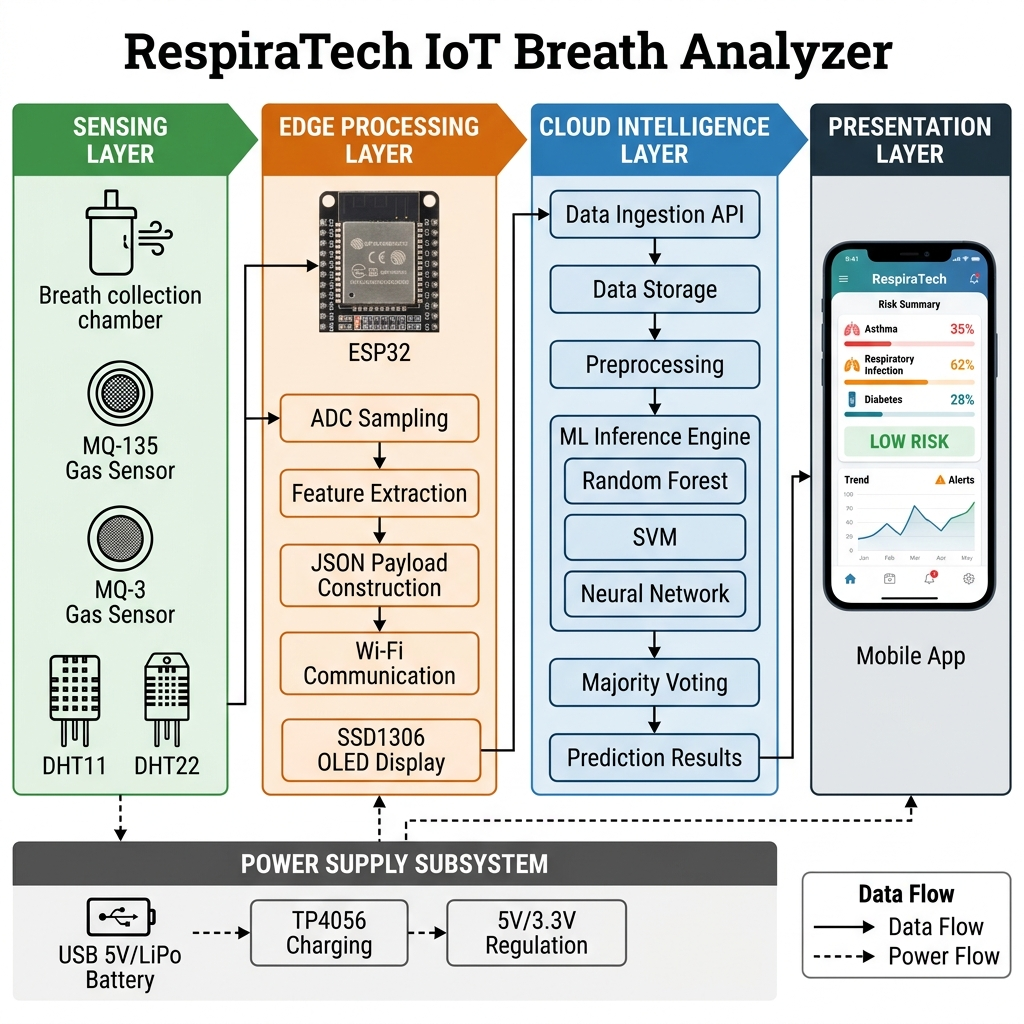
\includegraphics[width=\textwidth]{images/system_architecture.png}
\caption{System Architecture Diagram -- RespiraTech Intelligent IoT and AI-Based Breath Analyzer}
\label{fig:system_architecture}
\end{figure}

% CHAPTER 7: EXPECTED OUTCOME
\chapter{Expected Outcome}

Upon successful completion of the project, the following functional outcomes and performance targets are expected to be achieved:

\section{Functional Outcomes}
\begin{itemize}[leftmargin=1.5cm]
\item A working prototype of the RespiraTech smart breath analyzer device that will capture exhaled breath samples through a dedicated collection chamber, measure VOC concentrations using the MQ-135 and MQ-3 gas sensor array, and wirelessly transmit the processed data to a cloud platform for AI-based disease prediction. The device will be portable, battery-powered, and operable through a simple push-button interface requiring no technical expertise from the user.

\item A cloud-based AI inference pipeline that will preprocess incoming sensor data, normalize readings with environmental compensation, and run the data through three machine learning classifiers (Random Forest, SVM, Neural Network) to generate disease risk predictions. The prediction results will include risk percentages for three disease categories: asthma, respiratory infections, and diabetes.

\item Three core health screening capabilities accessible through a single breath test:
\begin{enumerate}
\item \textbf{Respiratory Disease Screening} --- The MQ-135 sensor will detect broad-spectrum VOC patterns associated with airway inflammation, detecting elevated levels of nitrogen oxides, aldehydes, and other respiratory biomarkers to assess asthma and respiratory infection risk.
\item \textbf{Diabetes Screening} --- The MQ-3 sensor will detect elevated acetone concentrations in breath that are characteristic of diabetic ketoacidosis. Breath acetone levels above 1.8 ppm will trigger elevated diabetes risk predictions.
\item \textbf{General Health Assessment} --- The combined sensor array data will provide an overall health status indicator based on the aggregate VOC profile, identifying deviations from healthy baseline patterns.
\end{enumerate}

\item A responsive mobile or web application that will display disease risk percentages, historical health trend charts, and automated alert notifications. The application will support multiple user profiles and provide exportable health reports for sharing with healthcare providers.

\item A local OLED display on the device that will show real-time sensor readings during breath capture, processing status indicators, and prediction results including disease risk percentages and overall health status (Low/Medium/High risk).

\item A complete data logging system that will store all breath test results with timestamps in the cloud database, enabling longitudinal health monitoring and trend analysis over weeks and months.
\end{itemize}

\section{Expected Performance Metrics}
The following performance metrics are anticipated based on the architectural design and component specifications:

\begin{table}[h]
\centering
\begin{tabular}{|l|c|c|}
\hline
\textbf{Metric} & \textbf{Target Value} & \textbf{Measurement Method} \\
\hline
ML Classification Accuracy & $>$ 80\% & 5-fold cross-validation \\
\hline
Breath Capture Duration & 10 seconds & Timer-controlled sampling \\
\hline
Cloud Processing Time & $<$ 3 seconds & Server-side timing \\
\hline
End-to-End Response Time & $<$ 15 seconds & Capture to OLED display \\
\hline
Wi-Fi Transmission Reliability & $>$ 99\% & 100-transmission test \\
\hline
Sensor Warm-Up Time & $<$ 3 minutes & After initial calibration \\
\hline
Battery Life (continuous) & $>$ 3 hours & Full operation with sensors \\
\hline
\end{tabular}
\caption{Expected Performance Metrics}
\end{table}

\section{System-Level Expectations}
\begin{itemize}[leftmargin=1.5cm]
\item \textbf{Sensor Sensitivity:} The MQ-135 is expected to detect VOC concentrations in the range of 10--1000 ppm, while the MQ-3 is expected to detect ethanol/acetone concentrations in the range of 0.04--4 mg/L. These ranges are sufficient to capture the biomarker concentration differences between healthy and diseased breath samples documented in the literature.

\item \textbf{Multi-Disease Screening:} The ensemble ML approach (Random Forest + SVM + Neural Network with majority voting) is expected to achieve higher accuracy than any individual classifier, based on established machine learning ensemble theory and results reported in the literature review.

\item \textbf{Environmental Compensation:} The inclusion of temperature and humidity data in the feature vector is expected to reduce false positive rates by 10--15\% compared to systems that do not compensate for ambient conditions, as gas sensor sensitivity is known to vary significantly with environmental factors.

\item \textbf{Data Security:} All data transmitted between the ESP32 and cloud platform will use HTTPS encryption, and user health data stored in the cloud will be access-controlled through authentication tokens, ensuring compliance with health data privacy best practices.

\item \textbf{Scalability:} The cloud-based architecture will enable the system to support multiple RespiraTech devices simultaneously, as each device communicates independently with the cloud platform via stateless REST API calls.
\end{itemize}

% CHAPTER 8: ADVANTAGES AND FUTURE SCOPE
\chapter{Advantages and Future Scope}

\section{Advantages}
The proposed RespiraTech breath analyzer system will offer the following significant advantages:

\begin{enumerate}[leftmargin=1.5cm]
\item \textbf{Non-Invasive Diagnostics:} The system will require only an exhaled breath sample for disease screening, completely eliminating the need for blood draws, needle pricks, or any other invasive procedures. This will make health screening painless, comfortable, and accessible to patients who avoid traditional diagnostics due to fear of needles or discomfort, including children and elderly individuals.

\item \textbf{Affordable Hardware:} The hardware prototype will use commercially available, low-cost electronic components including the ESP32 microcontroller, MQ-series gas sensors, and DHT environmental sensors. This will make the system significantly more affordable than clinical diagnostic equipment such as spirometers, blood gas analyzers, and mass spectrometers, enabling deployment in resource-constrained healthcare settings.

\item \textbf{Multi-Disease Screening:} Unlike most existing breath analysis systems that target a single disease, RespiraTech will screen for multiple conditions (asthma, respiratory infections, diabetes) from a single breath sample using the multi-sensor array and ensemble ML classification approach. This comprehensive screening capability will maximize the diagnostic value of each breath test.

\item \textbf{Real-Time Results:} Disease risk predictions will be delivered within 15 seconds of breath capture, compared to hours or days typically required for laboratory-based diagnostic tests. This rapid turnaround will enable immediate clinical decision-making and patient counselling, particularly valuable in emergency and point-of-care settings.

\item \textbf{Continuous Health Monitoring:} The cloud-based data storage and mobile/web application will enable users to perform regular breath tests and track their health trends over time. This longitudinal monitoring capability will support early detection of gradual health deterioration, medication effectiveness tracking, and recovery progress assessment.

\item \textbf{Remote Healthcare Accessibility:} The portable, battery-powered design with cloud-based AI processing will enable health screening in locations lacking clinical infrastructure. Community health workers in rural areas will be able to carry the device and screen patients during home visits, transmitting results to remote physicians for telemedicine consultation.

\item \textbf{AI-Enhanced Accuracy:} The ensemble machine learning approach (combining Random Forest, SVM, and Neural Network classifiers with majority voting) is expected to achieve higher prediction accuracy than any single algorithm or threshold-based approach, reducing false positives and false negatives compared to simpler diagnostic methods.

\item \textbf{Scalable and Extensible Architecture:} The cloud-based processing architecture will allow new ML models trained on expanded datasets to be deployed without modifying the hardware device. As more breath data is collected and labelled, the AI models can be retrained and improved, continuously enhancing the system's diagnostic capabilities.
\end{enumerate}

\section{Future Scope}
The modular architecture of the proposed system will enable several enhancements in future iterations:

\begin{enumerate}[leftmargin=1.5cm]
\item \textbf{Additional Sensor Integration:} Incorporating specialized gas sensors such as the MQ-7 (carbon monoxide), MQ-4 (methane), and MQ-8 (hydrogen) will expand the VOC detection spectrum and enable screening for additional diseases including liver disease (elevated hydrogen), gastrointestinal disorders (elevated methane), and carbon monoxide poisoning.

\item \textbf{Deep Learning Models:} Implementing advanced deep learning architectures such as Convolutional Neural Networks (CNNs) applied to raw sensor time-series data and Long Short-Term Memory (LSTM) networks for temporal pattern recognition will potentially improve classification accuracy beyond 90\% by capturing complex non-linear relationships in the sensor data.

\item \textbf{Edge AI Processing:} Deploying lightweight ML models (TensorFlow Lite Micro) directly on the ESP32-S3 (which supports vector instructions) will enable offline disease prediction without requiring cloud connectivity, making the system functional in areas with no internet access.

\item \textbf{Bluetooth Low Energy (BLE) Integration:} Adding BLE connectivity will enable direct communication with smartphones without requiring a Wi-Fi network, allowing the system to function through a companion mobile app in environments lacking Wi-Fi infrastructure.

\item \textbf{Clinical Trial Validation:} Conducting controlled clinical trials with hospital-verified patient diagnoses will provide validated training data for the ML models, improving prediction reliability and potentially enabling the system to receive medical device certification for clinical use.

\item \textbf{Cancer Screening Capability:} Research has shown that specific VOC biomarkers (aldehydes, alkanes, aromatic compounds) are associated with lung, breast, and colorectal cancers. With the addition of more sensitive sensors and expanded training data, future versions could incorporate preliminary cancer screening capabilities.

\item \textbf{Federated Learning:} Implementing federated learning across multiple deployed RespiraTech devices will allow the ML models to be improved using real-world data from diverse populations without centralizing sensitive health data, addressing both accuracy and privacy concerns simultaneously.

\item \textbf{Integration with Electronic Health Records (EHR):} Developing APIs for integration with hospital EHR systems (HL7 FHIR standard) will enable seamless incorporation of breath test results into patient medical records, supporting comprehensive clinical decision-making.
\end{enumerate}

% CHAPTER 9: CONCLUSION AND REFERENCES
\chapter{Conclusion}

This project proposes the design and implementation of RespiraTech, an intelligent IoT and AI-based breath analyzer system for early disease prediction in healthcare. The system will address the critical need for affordable, non-invasive, and accessible diagnostic tools by leveraging the established scientific principle that volatile organic compounds (VOCs) in exhaled human breath serve as biomarkers for various respiratory and metabolic diseases.

The hardware platform will be built around the ESP32 microcontroller interfaced with a dual gas sensor array comprising the MQ-135 (broad-spectrum VOC detection) and MQ-3 (ethanol/acetone-specific detection), supplemented by DHT11/DHT22 environmental sensors for temperature and humidity compensation. The multi-sensor approach will enable comprehensive breath profiling that captures a broader spectrum of VOC information than single-sensor configurations, improving the reliability and specificity of disease detection.

The cloud-based AI pipeline represents the core technical contribution of this project. By transmitting sensor data from the ESP32 to a cloud platform (ThingSpeak/Firebase) and applying an ensemble of three machine learning classifiers---Random Forest, Support Vector Machine, and Neural Network---with majority voting and confidence-weighted probability averaging, the system will generate disease risk predictions for asthma, respiratory infections, and diabetes from a single breath sample. This multi-model ensemble approach is expected to achieve classification accuracy above 80\%, exceeding the performance of any individual classifier.

The data flow architecture will follow a five-stage pipeline: breath capture (10-second sensor sampling at 10 Hz), local feature extraction (11 statistical features computed on the ESP32), cloud transmission (HTTP POST with API authentication), AI inference (ensemble ML classification), and result delivery (OLED display and mobile/web application). The complete end-to-end process is designed to complete within 15 seconds, providing near-real-time health screening results.

The user interface will deliver prediction results through dual channels: a local SSD1306 OLED display on the device showing immediate risk percentages and health status indicators, and a responsive mobile/web application providing comprehensive health dashboards, historical trend charts, and automated alert notifications for anomalous readings.

The RespiraTech system will demonstrate that the combination of affordable IoT sensor hardware, cloud-based machine learning analytics, and user-friendly health applications can provide meaningful disease screening capabilities at a fraction of the cost of clinical diagnostic equipment. By making early disease detection portable, non-invasive, and accessible, the system has the potential to improve healthcare outcomes in underserved communities where access to clinical diagnostic facilities remains limited. The modular and extensible architecture will ensure that the system can be enhanced with additional sensors, improved AI models, and expanded disease screening capabilities as the technology matures and more validated training data becomes available.

% =====================================================================
% REFERENCES
% =====================================================================
\chapter{References}

\begin{enumerate}[leftmargin=1.5cm]
\item A. Amann, W. Miekisch, J. Schubert, B. Buszewski, T. Ligor, T. Jezierski, J. Pleil, and T. Risby, ``Analysis of Exhaled Breath for Disease Detection,'' \textit{Annual Review of Analytical Chemistry}, vol. 7, pp. 455--482, 2014.

\item M. V. Farraia, J. Cavaleiro Rufo, I. Paciencia, F. Mendes, L. Delgado, and A. Moreira, ``The Electronic Nose Technology in Clinical Diagnosis: A Systematic Review,'' \textit{Porto Biomedical Journal}, vol. 4, no. 4, pp. 1--8, 2019.

\item M. K. Nakhleh, H. Amal, R. Jeries, et al., ``Diagnosis and Classification of 17 Diseases from 1404 Subjects via Pattern Analysis of Exhaled Molecules,'' \textit{ACS Nano}, vol. 11, no. 1, pp. 112--125, 2017.

\item S. Dragonieri, G. Pennazza, P. Carratu, and O. Resta, ``Electronic Nose Technology in Respiratory Diseases,'' \textit{Lung}, vol. 195, no. 2, pp. 157--165, 2017.

\item M. Righettoni, A. Tricoli, and S. E. Pratsinis, ``Si:WO$_3$ Sensors for Highly Selective Detection of Acetone for Easy Diagnosis of Diabetes by Breath Analysis,'' \textit{Analytical Chemistry}, vol. 82, no. 9, pp. 3581--3587, 2010.

\item V. A. Binson, M. Subramoniam, Y. Sunny, and L. Mathew, ``Prediction of Pulmonary Diseases with Electronic Nose Using SVM and XGBoost,'' \textit{IEEE Sensors Journal}, vol. 21, no. 18, pp. 20886--20895, 2021.

\item N. Dey, A. S. Ashour, F. Shi, S. J. Fong, and J. M. R. S. Tavares, ``Medical Cyber-Physical Systems: A Survey,'' \textit{Journal of Medical Systems}, vol. 42, no. 4, pp. 74, 2018.

\item Espressif Systems, ``ESP32 Technical Reference Manual,'' Version 4.6, 2022. [Online]. Available: \url{https://www.espressif.com/sites/default/files/documentation/esp32_technical_reference_manual_en.pdf}

\item Zhengzhou Winsen Electronics Technology, ``MQ-135 Gas Sensor Module Manual,'' Version 1.4, 2014. [Online]. Available: \url{https://www.winsen-sensor.com}

\item ThingSpeak, ``IoT Analytics Platform Documentation,'' MathWorks, 2024. [Online]. Available: \url{https://thingspeak.com/docs}

\item F. Pedregosa, G. Varoquaux, A. Gramfort, et al., ``Scikit-learn: Machine Learning in Python,'' \textit{Journal of Machine Learning Research}, vol. 12, pp. 2825--2830, 2011.

\item World Health Organization, ``Tracking Universal Health Coverage: 2021 Global Monitoring Report,'' WHO and World Bank, Geneva, 2021.
\end{enumerate}


\end{document}
